\chapter{Experimental Protocols}
\label{app:experimental}
	\doublespacing
	Each of the protocols detailed here were carried out on a Siemens ACUSON S2000\textsuperscript{\texttrademark}\ portable ultrasound machine with a Siemens 9L4 transducer on a CIRS Elasticity QA Phantom model 049 as shown in Fig. \ref{fig:experimental_photo}.

 	\singlespacing
	\begin{figure*}[!htb]
		\centering
		\begin{tikzpicture}
			\node at (0, 0) {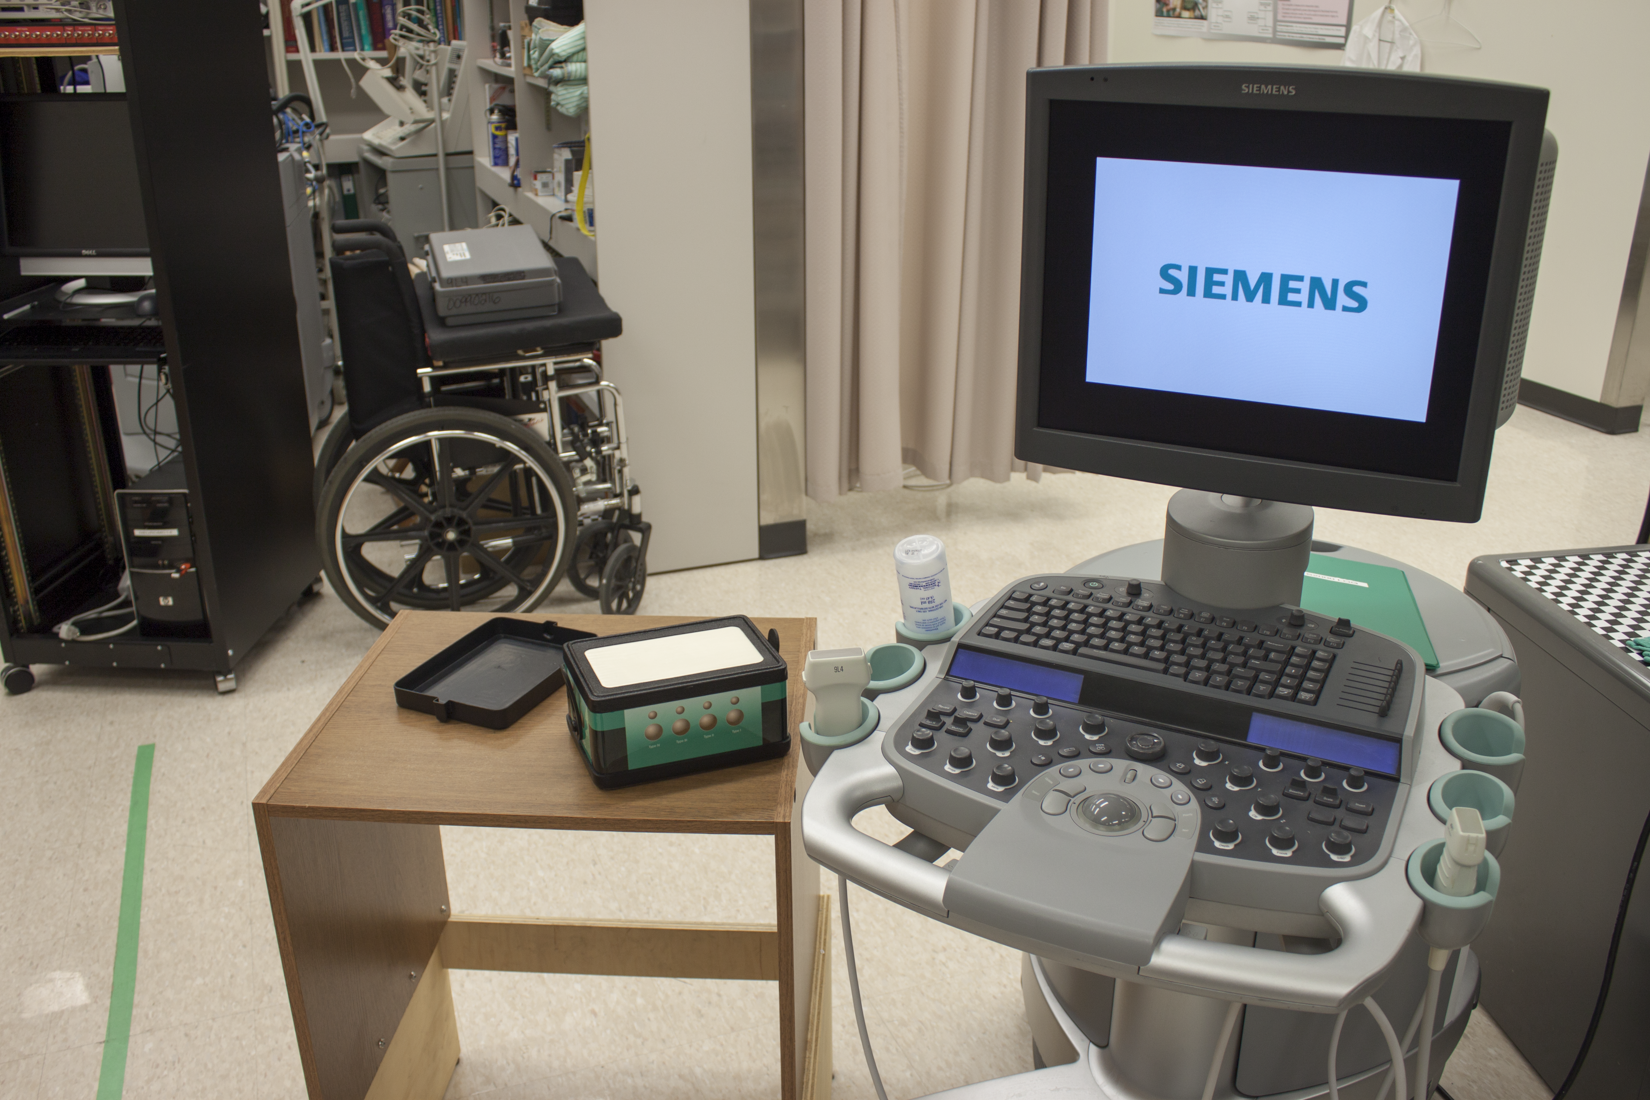
\includegraphics[width=\textwidth]{assets/experimental_setup.png}};

			% the phantom
			\draw[pc1,->,ultra thick] (-0.5, 1) -- (-1,-0.9);
			\draw (-0.5, 1) node[above,text width=1in,align=center,fill=white,rounded corners=3pt,draw=pc1,ultra thick]{\color{black}\footnotesize CIRS Elasticity QA Phantom model 049};

			% the probe
			\draw[pc2,->,ultra thick] (-2, -3.15) -- (0, -1.3);
			\draw (-2, -3.15) node[below,text width=1in,align=center,fill=white,rounded corners=3pt,draw=pc2,ultra thick]{\color{black}\footnotesize 9L4 Transducer};

			% the ultrasound machine
			\draw[pc3,->,ultra thick] (-0.5, 4) -- (2.5, 2.5);
			\draw (-0.5, 4) node[left,text width=1.5in,align=center,fill=white,rounded corners=3pt,draw=pc3,ultra thick]{\color{black}\footnotesize Siemens ACUSON S2000\textsuperscript{\texttrademark}\ portable ultrasound machine};
		\end{tikzpicture}
		\caption[]{Experimental setup showing the ultrasound machine, probe, and phantom model.}
		\label{fig:experimental_photo}
	\end{figure*}

	\section{Quasi-Static Ultrasound Elastography}
		\label{appsec:experimental_quasistatic}
		\begin{enumerate}
			\item Apply a layer of ultrasound gel to the active transducer area
			\item Begin a new ``2D'' imaging sequence on the machine using the ``Breast'' preset
			\item \label{itqs:position_transducer} Position the transducer for the desired lesion
			\begin{enumerate}
				\item Note the planar location of the lesion denoted on the sides of the phantom model
				\item Place the active component on the surface of the phantom model
				\item Align the transducer so as to intersect the lesion's planar location in a perpendicular manner
			\end{enumerate}
			\item Adjust the depth of the image to reach the full domain depth of the phantom model (approximately \SI{7.5}{\cm})
			\item Save the current screen
			\item Manually indent the transducer into the tissue by approximately \SI{0.5}{\cm}
			\item \label{itqs:save_second_image} Save the current screen
			\item Repeat steps \ref{itqs:position_transducer} -- \ref{itqs:save_second_image} until all desired images have been acquired
			\item Export the images to ``USB in PC format''
			\item Import the images into MATLAB\textsuperscript{\textregistered}
			\begin{enumerate}
				\item Crop the images so only the imaged domain is visible
			\end{enumerate}
			\item Process the cropped images using a strain estimation algorithm
		\end{enumerate}

	\section{Acoustic Radiation Force Impulse Imaging}
		\label{appsec:experimental_arfi}
		\begin{enumerate}
			\item Apply a layer of ultrasound gel to the active transducer area
			\item Begin a new ``2D'' imaging sequence on the machine using the ``Breast'' preset
			\item \label{itar:position_transducer} Position the transducer for the desired lesion
			\begin{enumerate}
				\item Note the planar location of the lesion denoted on the sides of the phantom model
				\item Place the active component on the surface of the phantom model
				\item Align the transducer so as to intersect the lesion's planar location in a perpendicular manner
			\end{enumerate}
			\item Adjust the depth of the image to reach the full domain depth of the phantom model (approximately \SI{7.5}{\cm})
			\item Using the ultrasound machine's trackball, select the ``Virtual Touch imaging'' button
			\item Ensure the elastogram colour map is a gradient from black to white
			\item Using the trackball and the ``Next'' button, adjust the position and size of the region of interest in order to fully capture the lesion and surrounding tissue
			\item Press the ``Update'' button and hold the transducer as motionless as possible while the scan completes
			\item Save the current screen
			\item \label{itar:unfreeze} Wait for the cooling process to complete then press the ``Freeze'' button to unfreeze the image
			\item Repeat steps \ref{itar:position_transducer} -- \ref{itar:unfreeze} until all desired images have been acquired
			\item Export the images to ``USB in PC format''
			\item Import the images into MATLAB\textsuperscript{\textregistered}
			\item Calculate the stiffness ratios by comparing the mean brightness of the elastograms inside the lesion to the mean brightness of the elastograms in an identical area located superior to the lesion
		\end{enumerate}

	\section{Shear Wave Speed Quantification}
		\label{appsec:experimental_shear}
		\begin{enumerate}
			\item Apply a layer of ultrasound gel to the active transducer area
			\item Begin a new ``2D'' imaging sequence on the machine using the ``Breast'' preset
			\item \label{itsh:position_transducer} Position the transducer for the desired lesion
			\begin{enumerate}
				\item Note the planar location of the lesion denoted on the sides of the phantom model
				\item Place the active component on the surface of the phantom model
				\item Align the transducer so as to intersect the lesion's planar location in a perpendicular manner
			\end{enumerate}
			\item Adjust the depth of the image to reach the full domain depth of the phantom model (approximately \SI{7.5}{\cm})
			\item Using the ultrasound machine's trackball, select the ``Virtual Touch Quantification imaging'' button
			\item Using the trackball, position the region of interest within the lesionous region
			\item Press the ``Update'' button and hold the transducer as motionless as possible while the scan completes
			\item Record the shear wave speed ($Vs$) of the interrogated region
			\item Wait for the cooling process to complete then press the ``Freeze'' button to unfreeze the image
			\item Using the trackball, position the region of interest outside the lesionous region
			\item Press the ``Update'' button and hold the transducer as motionless as possible while the scan completes
			\item Record the shear wave speed ($Vs$) of the interrogated region
			\item \label{itsh:unfreeze} Wait for the cooling process to complete then press the ``Freeze'' button to unfreeze the image
			\item Repeat steps \ref{itsh:position_transducer} -- \ref{itsh:unfreeze} until all desired lesions have been investigated
		\end{enumerate}